\begin{frame}
  For any given gene, the UMI count \(X_j\) in the cell \(j\),   \(S_j\) is the
  scale factor for the cell \(j\), which reflect the sequencing depth in the
  cell \(j\). 
  \begin{align}
    X_{j} &\sim {\it Poisson}(\lambda) \\
    X_{j} &\sim {\it Poisson}(\myemph{S_j}\cdot\tilde{\lambda}) \\
    X_{j} &\sim {\it PoissonlogNormal}(\mu, \sigma^2) \nonumber \\
         &= \int_{\lambda} Poisson(X|\myemph{S_j}\cdot \lambda)\cdot logNormal(\lambda | \mu,\sigma^2) \\
    X_{j} &\sim {\it Negative Binomial} (\myemph{S_j}\cdot\mu, \phi)
  \end{align}
  \begin{itemize}
\item
  In NB distribution, we use the mean \(\mu\) and
  dispersion \(\phi\) (namely \(r\)) , and then the variance \(\sigma^2 = \mu +
  \mu^2/\phi\), and the success probability \(p = \frac{\mu}{\mu + \phi}\).
\item
  NB can be treated as Gamma-Poisson mixture, i.e., \({\scriptstyle NB(\mu,\phi)=\int_\lambda
  Poisson(\lambda)Gamma(\phi, \phi/\mu)}\), in which, \(\phi\) is the shape, and
  \(\phi/\mu\) is the rate parameter in Gamma distribution.
\end{itemize}
\end{frame}

\begin{frame}{One cell subpopulation from one individual}
  \begin{table}
    \centering
    \begin{tabular}{c|c|c|c|c|c|c}
      Gene & Obs & Poi & Pois & Poilognm & Poislognm & NB \\
      \hline
      CCL4L1    & 0.840& 0.813& 0.824& 0.843& 0.850& 0.842 \\
      CCL4L2    & 0.837& 0.810& 0.822& 0.840& 0.847& 0.839 \\
      CCL3L1    & 0.729& \mywarn{0.403}& \mywarn{0.429}& 0.727& 0.734& 0.737 \\
      CCL3L3    & 0.729& \mywarn{0.404}& \mywarn{0.430}& 0.727& 0.734& 0.736 \\
      MIR155HG  & 0.961& 0.953& 0.956& 0.960& 0.962& 0.961 \\
      TNFRSF4   & 0.958& 0.959& 0.962& 0.959& 0.962& 0.959 \\
      ICAM1     & 0.952& 0.938& 0.942& 0.951& 0.953& 0.952 \\
      NA.499    & 0.971& 0.971& 0.973& 0.971& 0.973& 0.971 \\
      HIST2H2AA4& 0.942& 0.944& 0.948& 0.944& 0.948& 0.944 \\
      HBB       & 0.661& \mywarn{0.445}& \mywarn{0.470}& 0.621& 0.624& \myemph{0.644} \\
      HBA2      & 0.785& \mywarn{0.670}& \mywarn{0.689}& 0.765& 0.768& 0.779 \\
      HBA1      & 0.875& 0.863& 0.871& 0.872& 0.878& 0.874 \\
      \hline
    \end{tabular}
    \caption{Zero ratio estimations for cells from Cluster 2, the individual R1}
  \end{table}
\end{frame}

\begin{frame}{Two cell subpopulations from one individuals}
  \begin{table}
    \centering
    \begin{tabular}{c|c|c|c|c|c|c}
      Gene & Obs & Poi & Pois & Poilognm & Poislognm & NB \\
      \hline
      CCL4L1    & 0.961& 0.953& 0.957& 0.960& 0.963& 0.961\\ 
      CCL4L2    & 0.960& 0.952& 0.956& 0.959& 0.962& 0.960\\
      CCL3L1    & 0.802& \mywarn{0.689}& \mywarn{0.711}& 0.798& 0.806& 0.803\\
      CCL3L3    & 0.802& \mywarn{0.689}& \mywarn{0.711}& 0.798& 0.806& 0.803\\
      MIR155HG  & 0.990& 0.989& 0.990& 0.990& 0.990& 0.990\\
      TNFRSF4   & 0.989& 0.989& 0.990& 0.989& 0.990& 0.989\\
      ICAM1     & 0.803& 0.783& 0.800& 0.802& 0.812& 0.803\\
      NA.499    & 0.920& 0.921& 0.928& 0.921& 0.928& 0.921\\
      HIST2H2AA4& 0.901& 0.900& 0.908& 0.901& 0.908& 0.901\\
      HBB       & 0.486& \mywarn{0.204}& \mywarn{0.234}& \mywarn{0.423}& \mywarn{0.412}& \myemph{0.457}\\
      HBA2      & 0.535& \mywarn{0.333}& \mywarn{0.365}& \mywarn{0.496}& \mywarn{0.492}& \myemph{0.520}\\
      HBA1      & 0.716& 0.653& 0.677& 0.705& 0.711& 0.712\\
      \hline 
    \end{tabular}
    \caption{Zero ratio estimations for cells from Cluster 1 and 2, the
      individual R1}
  \end{table}
\end{frame}

\begin{frame}{One cell subpopulation from all the individuals}
  \begin{table}
    \centering
    \begin{tabular}{c|c|c|c|c|c|c}
      Gene & Obs & Poi & Pois & Poilognm & Poislognm & NB \\
      \hline
      CCL4L1    & 0.953& 0.946& 0.958& 0.953& 0.962& 0.953\\ 
      CCL4L2    & 0.952& 0.945& 0.957& 0.952& 0.961& 0.953\\
      CCL3L1    & 0.925& \mywarn{0.871}& \mywarn{0.899}& 0.924& 0.934& 0.925\\
      CCL3L3    & 0.925& \mywarn{0.871}& \mywarn{0.899}& 0.924& 0.934& 0.925\\
      MIR155HG  & 0.985& 0.984& 0.987& 0.985& 0.988& 0.985\\
      TNFRSF4   & 0.978& 0.977& 0.982& 0.978& 0.982& 0.978\\
      ICAM1     & 0.965& 0.962& 0.971& 0.965& 0.972& 0.965\\
      NA.499    & 0.987& 0.987& 0.990& 0.987& 0.990& 0.987\\
      HIST2H2AA4& 0.948& 0.945& 0.957& 0.948& 0.958& 0.948\\
      HBB       & 0.911& \mywarn{0.469}& \mywarn{0.557}& \mywarn{0.892}& 0.907& \myemph{0.911}\\ 
      HBA2      & 0.934& \mywarn{0.763}& \mywarn{0.811}& 0.921& 0.932& 0.933\\
      HBA1      & 0.941& \mywarn{0.867}& \mywarn{0.895}& 0.936& 0.945& 0.941\\
     \hline 
    \end{tabular}
    \caption{Zero ratio estimations for cells from Cluster2, 10 individuals.}
  \end{table}
  
\end{frame}


\begin{frame}{Two cell subpopulations from all the individuals}
  \begin{table}
    \centering
    \begin{tabular}{c|c|c|c|c|c|c}
      Gene & Obs & Poi & Pois & Poilognm & Poislognm & NB \\
      \hline
      CCL4L1    & 0.969& 0.965& 0.974& 0.969& 0.975& 0.969\\ 
      CCL4L2    & 0.969& 0.964& 0.974& 0.969& 0.975& 0.969\\
      CCL3L1    & 0.857& \mywarn{0.761}& 0.819& 0.856& 0.873& 0.858\\
      CCL3L3    & 0.857& \mywarn{0.761}& 0.819& 0.856& 0.873& 0.858\\
      MIR155HG  & 0.991& 0.990& 0.993& 0.990& 0.992& \mywarn{NA}   \\
      TNFRSF4   & 0.986& 0.985& 0.989& 0.986& 0.989& 0.986\\
      ICAM1     & 0.873& 0.857& 0.893& 0.871& 0.897& 0.872\\
      NA.499    & 0.926& 0.916& 0.938& 0.926& 0.941& 0.926\\
      HIST2H2AA4& 0.901& 0.887& 0.916& 0.901& 0.921& 0.901\\
      HBB       & 0.823& \mywarn{0.289}& \mywarn{0.403}& 0.812& 0.819& 0.823\\
      HBA2      & 0.846& \mywarn{0.583}& \mywarn{0.674}& 0.838& 0.844& 0.844\\
      HBA1      & 0.890& 0.775& 0.830& 0.887& 0.898& 0.890\\
    \end{tabular}
    \caption{Zero ratio estimation for cells from Cluster 1 and 2, 10
      individuals.}
  \end{table}
\end{frame}


\begin{frame}
  \begin{figure}
    \centering
    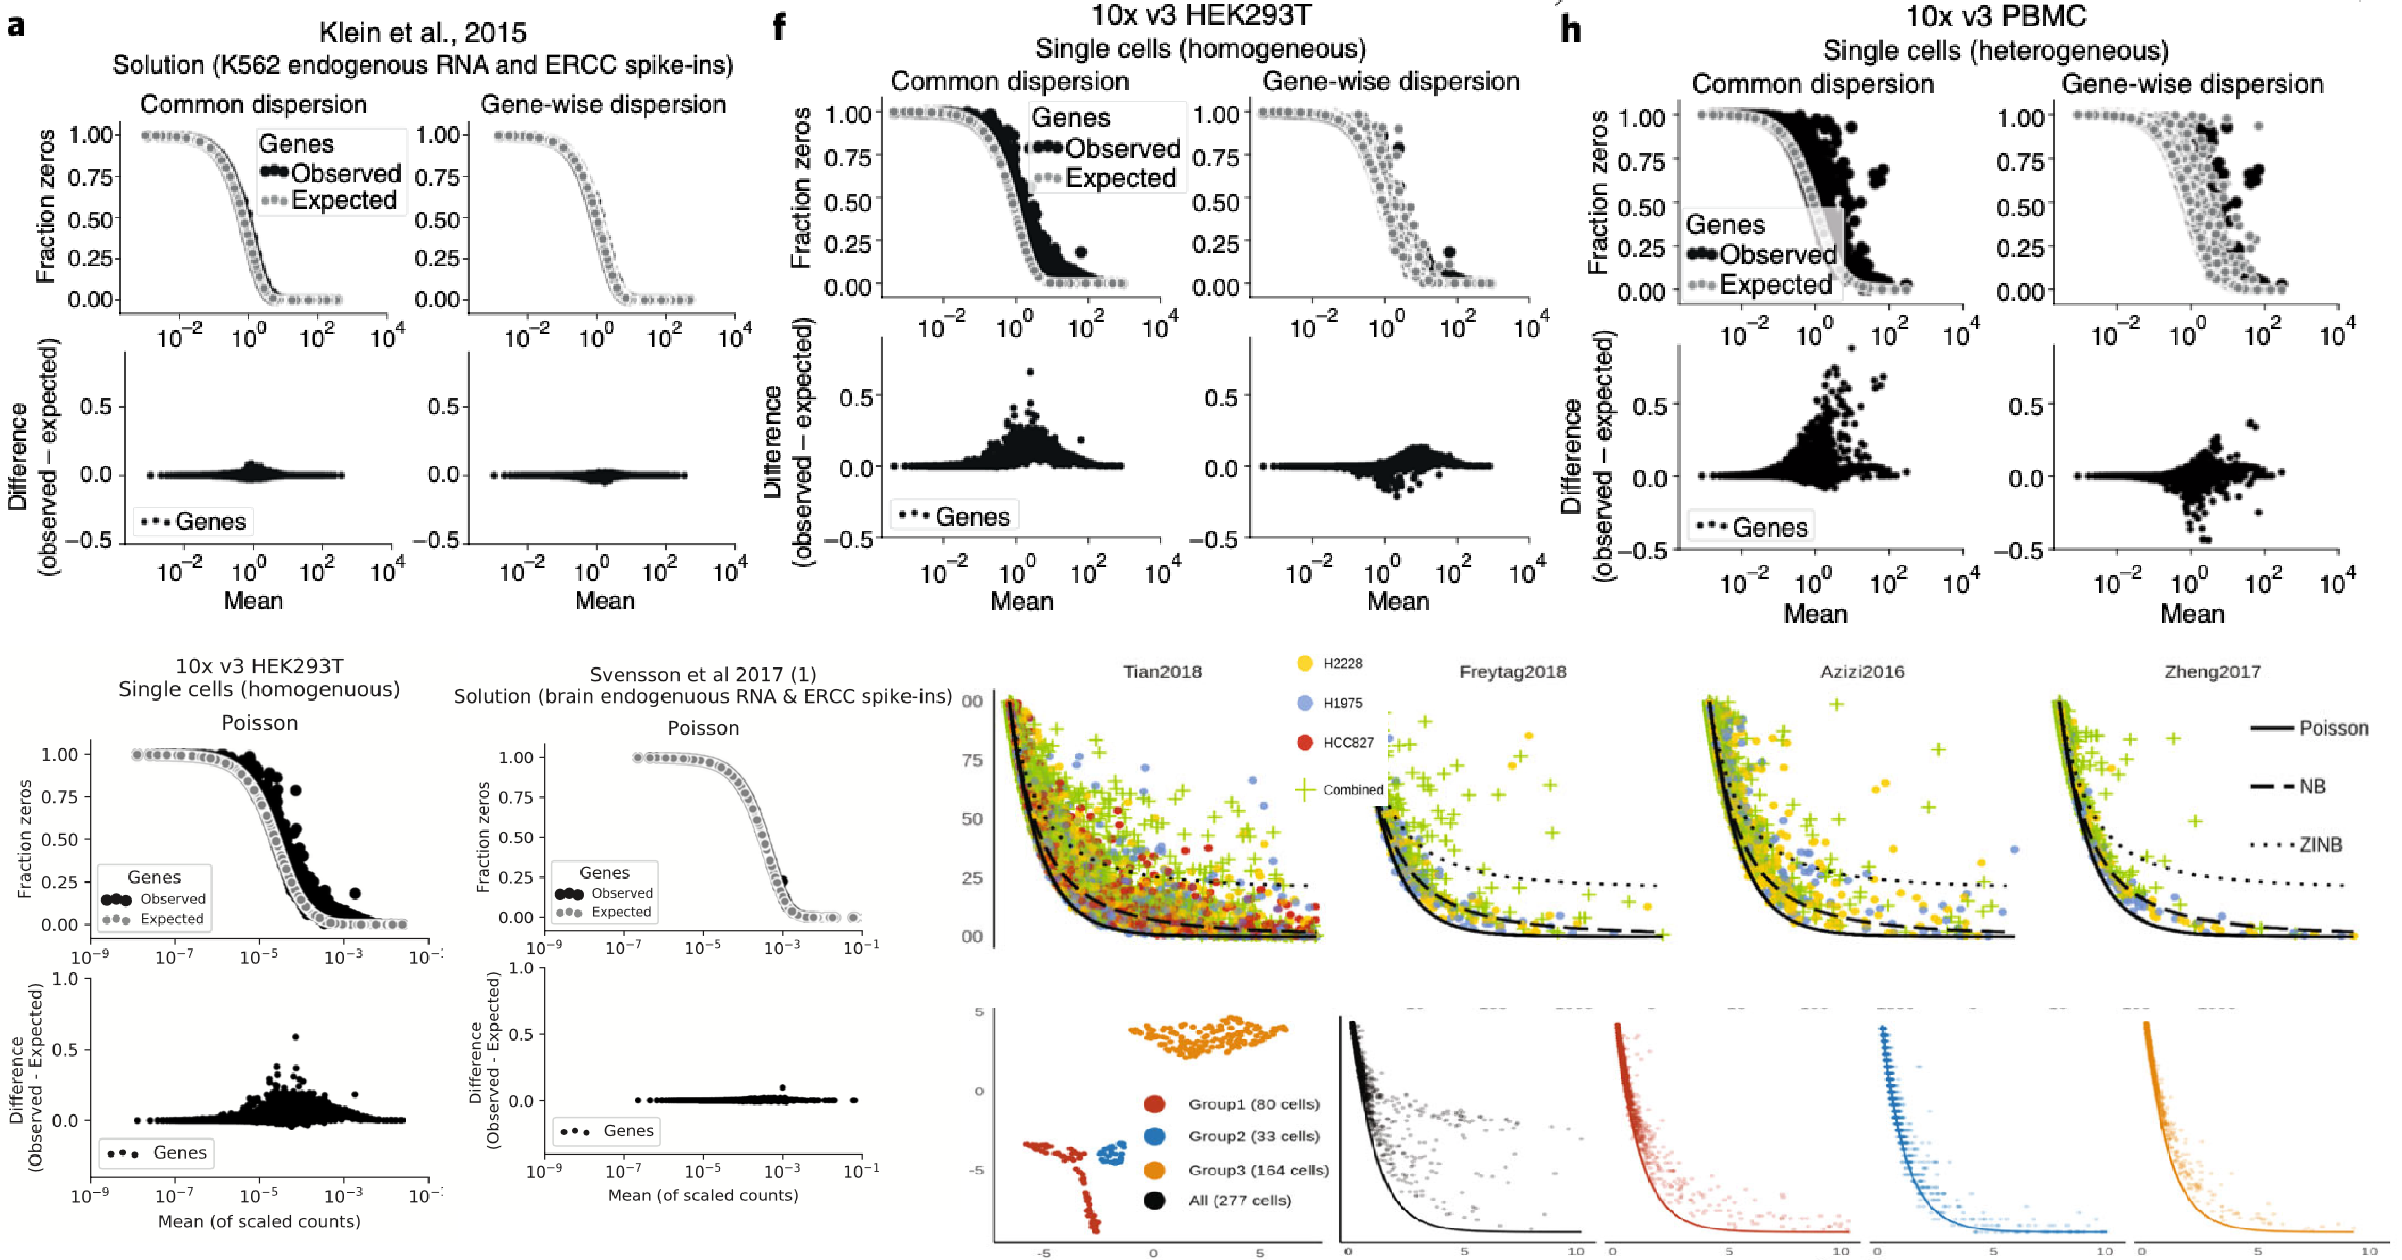
\includegraphics[width = \textwidth]{not_tech_zero_inflation}
    \caption{Observed and expected zeros with NB, Poisson or Poisson with scaled
    mean. Grey figures from \cite{svensson2020droplet}; color
    figures from \cite{kim2020demystifying}.}
  \end{figure}
\end{frame}

\begin{frame}
  \frametitle{Modeling scRNAseq Using Negative Binomial}
  \begin{itemize}
  \item
    We need the dispersion \(\phi\) for each gene to model the variance of gene
    expression 
    due to heterogeneity. In reality, we cannot get a group of homogeneous
    cells\footnote{Cell annotation itself is now a really hot topic in scRNAseq
      data analysis.}. Meanwhile, we can estimate \(\phi\) in each gene by sharing
    the same prior since we understand it will reflect the character of a given
    cell sub-population.
  \item
    Like DESeq2 \cite{love2014moderated} for bulkRNAseq DE analysis, we model
    the mean \(\mu\) across different conditions and different samples.
  \item
    We use Bayesian modeling since it could be more robust than usual MLE
    estimation. The posterior distribution about the parameters can tell us lots
    of information.
  \end{itemize}
\end{frame}